\documentclass[]{book}
\usepackage{lmodern}
\usepackage{amssymb,amsmath}
\usepackage{ifxetex,ifluatex}
\usepackage{fixltx2e} % provides \textsubscript
\ifnum 0\ifxetex 1\fi\ifluatex 1\fi=0 % if pdftex
  \usepackage[T1]{fontenc}
  \usepackage[utf8]{inputenc}
\else % if luatex or xelatex
  \ifxetex
    \usepackage{mathspec}
  \else
    \usepackage{fontspec}
  \fi
  \defaultfontfeatures{Ligatures=TeX,Scale=MatchLowercase}
\fi
% use upquote if available, for straight quotes in verbatim environments
\IfFileExists{upquote.sty}{\usepackage{upquote}}{}
% use microtype if available
\IfFileExists{microtype.sty}{%
\usepackage{microtype}
\UseMicrotypeSet[protrusion]{basicmath} % disable protrusion for tt fonts
}{}
\usepackage[margin=1in]{geometry}
\usepackage{hyperref}
\hypersetup{unicode=true,
            pdftitle={EPsy 8251 Notes},
            pdfauthor={Andrew Zieffler},
            pdfborder={0 0 0},
            breaklinks=true}
\urlstyle{same}  % don't use monospace font for urls
\usepackage{natbib}
\bibliographystyle{plainnat}
\usepackage{color}
\usepackage{fancyvrb}
\newcommand{\VerbBar}{|}
\newcommand{\VERB}{\Verb[commandchars=\\\{\}]}
\DefineVerbatimEnvironment{Highlighting}{Verbatim}{commandchars=\\\{\}}
% Add ',fontsize=\small' for more characters per line
\usepackage{framed}
\definecolor{shadecolor}{RGB}{248,248,248}
\newenvironment{Shaded}{\begin{snugshade}}{\end{snugshade}}
\newcommand{\AlertTok}[1]{\textcolor[rgb]{0.94,0.16,0.16}{#1}}
\newcommand{\AnnotationTok}[1]{\textcolor[rgb]{0.56,0.35,0.01}{\textbf{\textit{#1}}}}
\newcommand{\AttributeTok}[1]{\textcolor[rgb]{0.77,0.63,0.00}{#1}}
\newcommand{\BaseNTok}[1]{\textcolor[rgb]{0.00,0.00,0.81}{#1}}
\newcommand{\BuiltInTok}[1]{#1}
\newcommand{\CharTok}[1]{\textcolor[rgb]{0.31,0.60,0.02}{#1}}
\newcommand{\CommentTok}[1]{\textcolor[rgb]{0.56,0.35,0.01}{\textit{#1}}}
\newcommand{\CommentVarTok}[1]{\textcolor[rgb]{0.56,0.35,0.01}{\textbf{\textit{#1}}}}
\newcommand{\ConstantTok}[1]{\textcolor[rgb]{0.00,0.00,0.00}{#1}}
\newcommand{\ControlFlowTok}[1]{\textcolor[rgb]{0.13,0.29,0.53}{\textbf{#1}}}
\newcommand{\DataTypeTok}[1]{\textcolor[rgb]{0.13,0.29,0.53}{#1}}
\newcommand{\DecValTok}[1]{\textcolor[rgb]{0.00,0.00,0.81}{#1}}
\newcommand{\DocumentationTok}[1]{\textcolor[rgb]{0.56,0.35,0.01}{\textbf{\textit{#1}}}}
\newcommand{\ErrorTok}[1]{\textcolor[rgb]{0.64,0.00,0.00}{\textbf{#1}}}
\newcommand{\ExtensionTok}[1]{#1}
\newcommand{\FloatTok}[1]{\textcolor[rgb]{0.00,0.00,0.81}{#1}}
\newcommand{\FunctionTok}[1]{\textcolor[rgb]{0.00,0.00,0.00}{#1}}
\newcommand{\ImportTok}[1]{#1}
\newcommand{\InformationTok}[1]{\textcolor[rgb]{0.56,0.35,0.01}{\textbf{\textit{#1}}}}
\newcommand{\KeywordTok}[1]{\textcolor[rgb]{0.13,0.29,0.53}{\textbf{#1}}}
\newcommand{\NormalTok}[1]{#1}
\newcommand{\OperatorTok}[1]{\textcolor[rgb]{0.81,0.36,0.00}{\textbf{#1}}}
\newcommand{\OtherTok}[1]{\textcolor[rgb]{0.56,0.35,0.01}{#1}}
\newcommand{\PreprocessorTok}[1]{\textcolor[rgb]{0.56,0.35,0.01}{\textit{#1}}}
\newcommand{\RegionMarkerTok}[1]{#1}
\newcommand{\SpecialCharTok}[1]{\textcolor[rgb]{0.00,0.00,0.00}{#1}}
\newcommand{\SpecialStringTok}[1]{\textcolor[rgb]{0.31,0.60,0.02}{#1}}
\newcommand{\StringTok}[1]{\textcolor[rgb]{0.31,0.60,0.02}{#1}}
\newcommand{\VariableTok}[1]{\textcolor[rgb]{0.00,0.00,0.00}{#1}}
\newcommand{\VerbatimStringTok}[1]{\textcolor[rgb]{0.31,0.60,0.02}{#1}}
\newcommand{\WarningTok}[1]{\textcolor[rgb]{0.56,0.35,0.01}{\textbf{\textit{#1}}}}
\usepackage{longtable,booktabs}
\usepackage{graphicx,grffile}
\makeatletter
\def\maxwidth{\ifdim\Gin@nat@width>\linewidth\linewidth\else\Gin@nat@width\fi}
\def\maxheight{\ifdim\Gin@nat@height>\textheight\textheight\else\Gin@nat@height\fi}
\makeatother
% Scale images if necessary, so that they will not overflow the page
% margins by default, and it is still possible to overwrite the defaults
% using explicit options in \includegraphics[width, height, ...]{}
\setkeys{Gin}{width=\maxwidth,height=\maxheight,keepaspectratio}
\IfFileExists{parskip.sty}{%
\usepackage{parskip}
}{% else
\setlength{\parindent}{0pt}
\setlength{\parskip}{6pt plus 2pt minus 1pt}
}
\setlength{\emergencystretch}{3em}  % prevent overfull lines
\providecommand{\tightlist}{%
  \setlength{\itemsep}{0pt}\setlength{\parskip}{0pt}}
\setcounter{secnumdepth}{5}
% Redefines (sub)paragraphs to behave more like sections
\ifx\paragraph\undefined\else
\let\oldparagraph\paragraph
\renewcommand{\paragraph}[1]{\oldparagraph{#1}\mbox{}}
\fi
\ifx\subparagraph\undefined\else
\let\oldsubparagraph\subparagraph
\renewcommand{\subparagraph}[1]{\oldsubparagraph{#1}\mbox{}}
\fi

%%% Use protect on footnotes to avoid problems with footnotes in titles
\let\rmarkdownfootnote\footnote%
\def\footnote{\protect\rmarkdownfootnote}

%%% Change title format to be more compact
\usepackage{titling}

% Create subtitle command for use in maketitle
\newcommand{\subtitle}[1]{
  \posttitle{
    \begin{center}\large#1\end{center}
    }
}

\setlength{\droptitle}{-2em}

  \title{EPsy 8251 Notes}
    \pretitle{\vspace{\droptitle}\centering\huge}
  \posttitle{\par}
    \author{Andrew Zieffler}
    \preauthor{\centering\large\emph}
  \postauthor{\par}
      \predate{\centering\large\emph}
  \postdate{\par}
    \date{2018-12-02}

\usepackage{booktabs}
\usepackage{amsthm}
\makeatletter
\def\thm@space@setup{%
  \thm@preskip=8pt plus 2pt minus 4pt
  \thm@postskip=\thm@preskip
}
\makeatother

\usepackage{amsthm}
\newtheorem{theorem}{Theorem}[chapter]
\newtheorem{lemma}{Lemma}[chapter]
\theoremstyle{definition}
\newtheorem{definition}{Definition}[chapter]
\newtheorem{corollary}{Corollary}[chapter]
\newtheorem{proposition}{Proposition}[chapter]
\theoremstyle{definition}
\newtheorem{example}{Example}[chapter]
\theoremstyle{definition}
\newtheorem{exercise}{Exercise}[chapter]
\theoremstyle{remark}
\newtheorem*{remark}{Remark}
\newtheorem*{solution}{Solution}
\begin{document}
\maketitle

{
\setcounter{tocdepth}{1}
\tableofcontents
}
\hypertarget{prerequisites}{%
\chapter{Prerequisites}\label{prerequisites}}

This is a \emph{sample} book written in \textbf{Markdown}. You can use
anything that Pandoc's Markdown supports, e.g., a math equation
\(a^2 + b^2 = c^2\).

The \textbf{bookdown} package can be installed from CRAN or Github:

\begin{Shaded}
\begin{Highlighting}[]
\KeywordTok{install.packages}\NormalTok{(}\StringTok{"bookdown"}\NormalTok{)}
\CommentTok{# or the development version}
\CommentTok{# devtools::install_github("rstudio/bookdown")}
\end{Highlighting}
\end{Shaded}

Remember each Rmd file contains one and only one chapter, and a chapter
is defined by the first-level heading \texttt{\#}.

To compile this example to PDF, you need XeLaTeX. You are recommended to
install TinyTeX (which includes XeLaTeX):
\url{https://yihui.name/tinytex/}.

\hypertarget{simple-descript}{%
\chapter{Simple Linear Regression---Description}\label{simple-descript}}

In this set of notes, you will begin your foray into regression
analysis. To do so, we will use the \emph{riverside.csv} data to examine
whether education level is related to income. The data come from
\citet{Lewis-Beck:2016} and contain five attributes collected from a
random sample of \(n=32\) employees working for the city of Riverview, a
hyopothetical midwestern city. The attributes include:

\begin{itemize}
\tightlist
\item
  \texttt{education}: Years of formal education
\item
  \texttt{income}: Annual income (in thousands of U.S. dollars)
\item
  \texttt{seniority}: Years of seniority
\item
  \texttt{gender}: Employee's gender
\item
  \texttt{male}: Dummy coded gender variable (0 = Female, 1 = Male)
\item
  \texttt{party}: Political party affiliation
\end{itemize}

\hypertarget{preparation}{%
\section{Preparation}\label{preparation}}

\begin{Shaded}
\begin{Highlighting}[]
\CommentTok{# Load libraries}
\KeywordTok{library}\NormalTok{(corrr)}
\KeywordTok{library}\NormalTok{(dplyr)}
\KeywordTok{library}\NormalTok{(ggplot2)}
\KeywordTok{library}\NormalTok{(readr)}
\KeywordTok{library}\NormalTok{(sm)}

\CommentTok{# Read in data}
\NormalTok{city =}\StringTok{ }\KeywordTok{read_csv}\NormalTok{(}\DataTypeTok{file =} \StringTok{"~/Documents/github/epsy-8251/data/riverside.csv"}\NormalTok{)}
\KeywordTok{head}\NormalTok{(city)}
\end{Highlighting}
\end{Shaded}

\begin{verbatim}
## # A tibble: 6 x 6
##   education income seniority gender  male party      
##       <int>  <dbl>     <int> <chr>  <int> <chr>      
## 1         8   37.4         7 male       1 Democrat   
## 2         8   26.4         9 female     0 Independent
## 3        10   47.0        14 male       1 Democrat   
## 4        10   34.2        16 female     0 Independent
## 5        10   25.5         1 female     0 Republican 
## 6        12   46.5        11 female     0 Democrat
\end{verbatim}

\hypertarget{data-exploration}{%
\section{Data Exploration}\label{data-exploration}}

Any analysis should start with an initial exploration of the data.
During this exploration, you should examine each of the variables that
you will be including in the regression analysis. This will help you
understand results you get in later analyses, and will also help
foreshadow potential problems with the analysis. For additional detail,
\href{https://www.analyticsvidhya.com/blog/2016/01/guide-data-exploration/}{this
blog post} describes initial ideas of data exploration reasonably well.
You could also refer to almost any introductory statistics text.

It is typical to begin by exploring the distribution of each variable
separately. These distributions are referred to as \emph{marginal
distributions}. After that, it is appropriate to explore the
relationships between the variables.

\hypertarget{income}{%
\subsection{Income}\label{income}}

To begin this exploration, we will examine the marginal distribution of
employees' incomes. We can plot a marginal distribution using the
\texttt{sm.density()} function from the \textbf{sm} package.

\begin{Shaded}
\begin{Highlighting}[]
\KeywordTok{sm.density}\NormalTok{(city}\OperatorTok{$}\NormalTok{income, }\DataTypeTok{xlab =} \StringTok{"Income"}\NormalTok{)}
\end{Highlighting}
\end{Shaded}

\begin{figure}
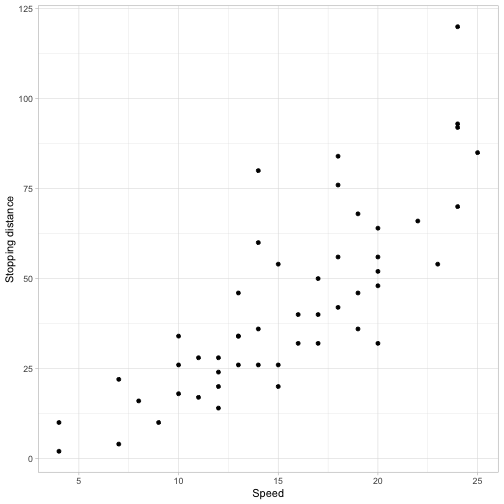
\includegraphics[width=0.5\linewidth]{bookdown-demo_files/figure-latex/unnamed-chunk-3-1} \caption{Density plot of employee incomes.}\label{fig:unnamed-chunk-3}
\end{figure}

This plot suggests that employees' incomes are unimodal with most
incomes between roughly \$50,000 and \$70,000. The rug at the bottom of
the plot (the small vertical line segments) show the 32 incomes from our
sample. The smallest income in the sample is about \$25,000 and the
largest income is over \$80,000. (We could find the exact values using
the \texttt{summary()} function.) This suggests there is a fair amount
of variation in the data.

To further summarize the distribution, it is typical to compute and
report summary statistics such as the mean and standard deviation. One
way to compute these values is to use functions from the \textbf{dplyr}
library.

\begin{Shaded}
\begin{Highlighting}[]
\NormalTok{city }\OperatorTok\StringTok{ }
\StringTok{  }\KeywordTok{summarize}\NormalTok{(}
    \DataTypeTok{M =} \KeywordTok{mean}\NormalTok{(income), }
    \DataTypeTok{SD =} \KeywordTok{sd}\NormalTok{(income)}
\NormalTok{    )}
\end{Highlighting}
\end{Shaded}

\begin{verbatim}
## # A tibble: 1 x 2
##       M    SD
##   <dbl> <dbl>
## 1  53.7  14.6
\end{verbatim}

Describing this variable we might write,

\begin{quote}
The marginal distribution of income is unimodal with a mean of 53.74
thousand dollars. There is variation in employees' salaries (SD = 14.55
thousand dollars).
\end{quote}

\hypertarget{education-level}{%
\subsection{Education Level}\label{education-level}}

We will also examine the distribution of the education level variable.

\begin{Shaded}
\begin{Highlighting}[]
\CommentTok{# Plot}
\KeywordTok{sm.density}\NormalTok{(city}\OperatorTok{$}\NormalTok{education, }\DataTypeTok{xlab =} \StringTok{"Education Level"}\NormalTok{)}
\end{Highlighting}
\end{Shaded}

\begin{figure}
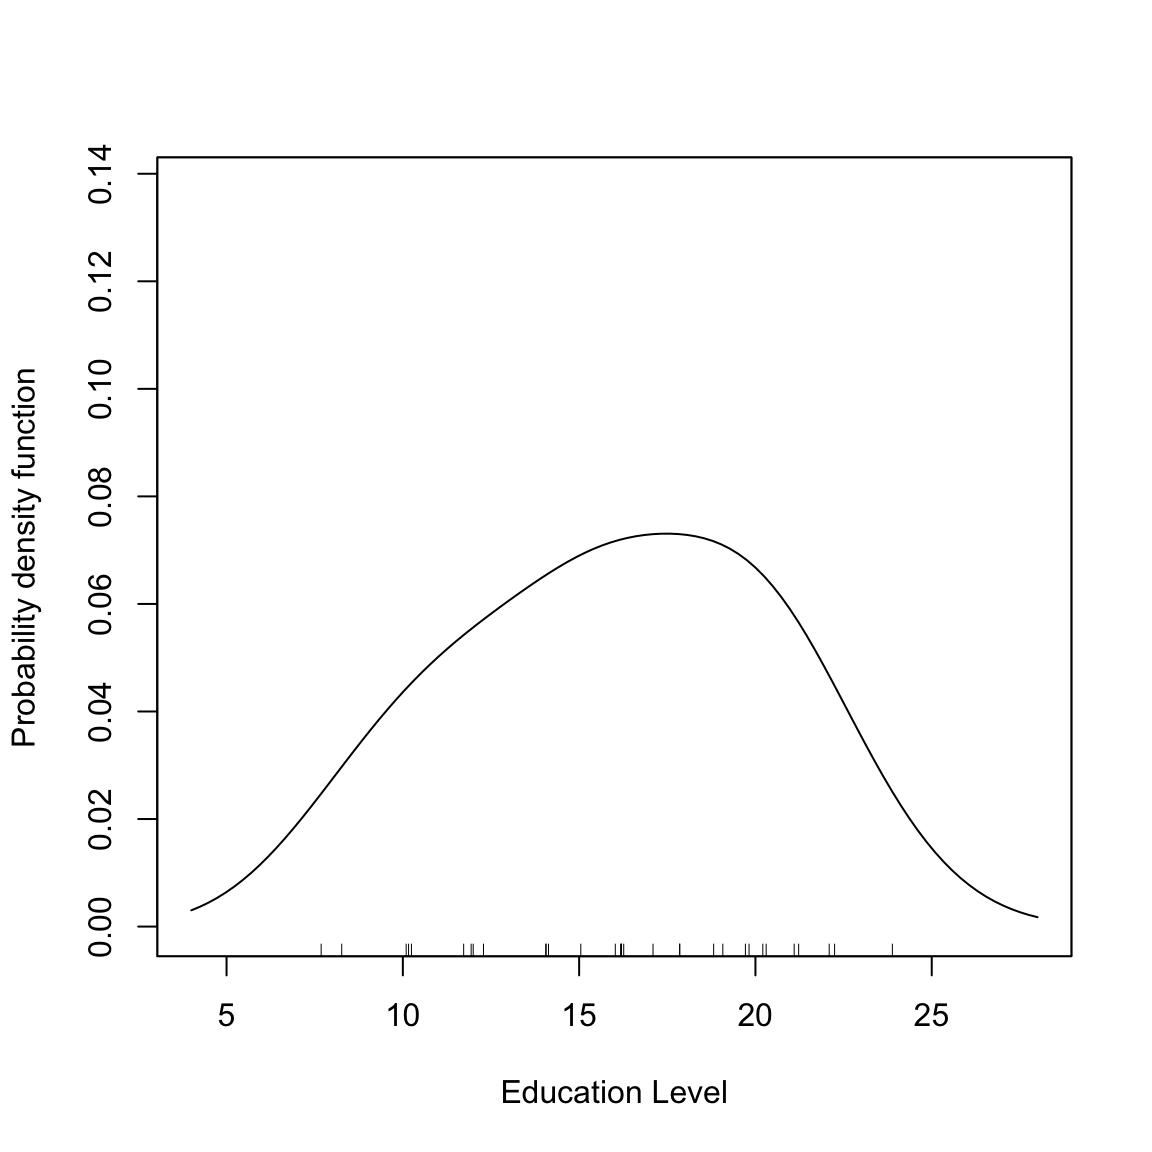
\includegraphics[width=0.5\linewidth]{bookdown-demo_files/figure-latex/unnamed-chunk-5-1} \caption{Density plot of employee education levels.}\label{fig:unnamed-chunk-5}
\end{figure}

Computing the mean and standard deviation:

\begin{Shaded}
\begin{Highlighting}[]
\CommentTok{# Summary statistics}
\NormalTok{city }\OperatorTok\StringTok{ }
\StringTok{  }\KeywordTok{summarize}\NormalTok{(}
    \DataTypeTok{M =} \KeywordTok{mean}\NormalTok{(education), }
    \DataTypeTok{SD =} \KeywordTok{sd}\NormalTok{(education)}
\NormalTok{    )}
\end{Highlighting}
\end{Shaded}

\begin{verbatim}
## # A tibble: 1 x 2
##       M    SD
##   <dbl> <dbl>
## 1    16  4.36
\end{verbatim}

Again, we might write,

\begin{quote}
The marginal distribution of education is unimodal with a mean of 16
years. There is variation in employees' level of education (SD = 4.4).
\end{quote}

\hypertarget{relationship-between-variables}{%
\section{Relationship Between
Variables}\label{relationship-between-variables}}

Although examining the marginal distributions is an important first step
in the analysis, those descriptions do not help us directly answer our
research question. To better understand the relationship between income
and education level we need to explore the distribution of income
(\(Y\)) as a function of education (\(X\)). To do this, we will create a
scatterplot of incomes versus education.

\hypertarget{scatterplot}{%
\subsection{Scatterplot}\label{scatterplot}}

Below, we use \texttt{ggplot()} to create a scatterplot.

\begin{Shaded}
\begin{Highlighting}[]
\KeywordTok{ggplot}\NormalTok{(}\DataTypeTok{data =}\NormalTok{ city, }\KeywordTok{aes}\NormalTok{(}\DataTypeTok{x =}\NormalTok{ education, }\DataTypeTok{y =}\NormalTok{ income)) }\OperatorTok{+}
\StringTok{  }\KeywordTok{geom_point}\NormalTok{() }\OperatorTok{+}
\StringTok{  }\KeywordTok{theme_bw}\NormalTok{() }\OperatorTok{+}
\StringTok{  }\KeywordTok{xlab}\NormalTok{(}\StringTok{"Education (in years)"}\NormalTok{) }\OperatorTok{+}
\StringTok{  }\KeywordTok{ylab}\NormalTok{(}\StringTok{"Income (in thousands of U.S. dollars)"}\NormalTok{)}
\end{Highlighting}
\end{Shaded}

\begin{figure}
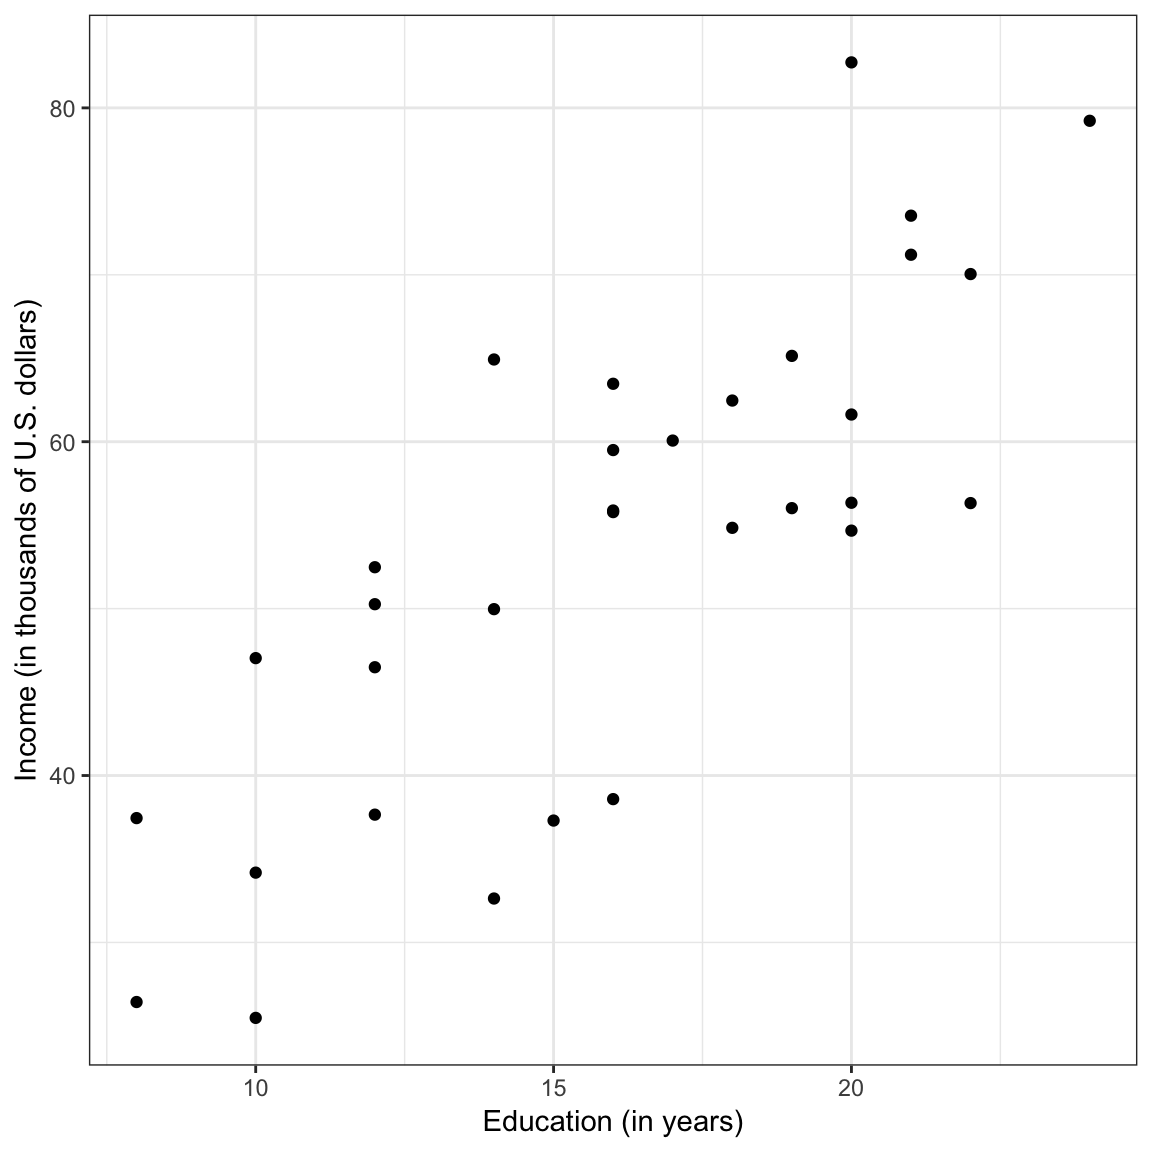
\includegraphics[width=0.5\linewidth]{bookdown-demo_files/figure-latex/unnamed-chunk-7-1} \caption{Scatterplot displaying the relationship between employee education levels and incomes.}\label{fig:unnamed-chunk-7}
\end{figure}

The plot suggests a relationship (at least for these employees) between
level of education and income. When describing the relationship we want
to touch on four characteristics of the relationship:

\begin{itemize}
\tightlist
\item
  Functional form (structure) of the relationship
\item
  Direction
\item
  Strength
\item
  Observations that do not fit the trend (outliers)
\end{itemize}

\hypertarget{correlation}{%
\subsection{Correlation}\label{correlation}}

To numerically summarize relationships between variables, we typically
compute correlation coefficients. The correlation coefficient is a
quantification of the direction and strength of the relationship. (It is
important to note that the correlation coefficient is only an
appropriate summarization of the relationship if the functional form of
the relationship is linear.)

To compute the correlation coefficient, we use the \texttt{correlate()}
function from the \textbf{corrr} package. We can use the dplyr-type
syntax to select the variables we want correlations between, and then
pipe that into the \texttt{correlate()} function. Typically the response
(or outcome) variable is the first variable provided in the
\texttt{select()} function, followed by the predictor.

\begin{Shaded}
\begin{Highlighting}[]
\CommentTok{# Load corrr package}
\KeywordTok{library}\NormalTok{(corrr)}

\CommentTok{# Compute correlation between income and education level}
\NormalTok{city }\OperatorTok
\StringTok{  }\KeywordTok{select}\NormalTok{(income, education) }\OperatorTok
\StringTok{  }\KeywordTok{correlate}\NormalTok{()}
\end{Highlighting}
\end{Shaded}

\begin{verbatim}
## 
## Correlation method: 'pearson'
## Missing treated using: 'pairwise.complete.obs'
\end{verbatim}

\begin{verbatim}
## # A tibble: 2 x 3
##   rowname   income education
##   <chr>      <dbl>     <dbl>
## 1 income    NA         0.795
## 2 education  0.795    NA
\end{verbatim}

When reporting the correlation coefficient is is conventional to use a
lower-case \(r\) and report the value to two decimal places. Subscripts
are also generally used to indicate the variables. For example,

\[
r_{\mathrm{education,~income}} = 0.79
\]

Combining the information culled from the scatterplot with that of the
correlation analysis, we could summarize the relationship between
education level and income as,

\begin{quote}
There is a strong, positive, linear relationship between education level
and income (\(r = .79\)). This suggests that city employees with lower
education levels tend to have lower incomes, on average, than employees
with higher education levels.
\end{quote}

\hypertarget{statistical-model}{%
\section{Statistical Model}\label{statistical-model}}

The analytic goal is to now describe the relationship using a
statistical model. Since the structure of the relationship between
education level and income seems reasonably linear, we will use a
\emph{linear model} to describe the data. We can express this model
mathematically as,

\[
Y_i = \beta_0 + \beta_1(X_i) + \epsilon_i.
\]

In this equation,

\begin{itemize}
\tightlist
\item
  \(Y_i\) is the outcome/response value; it has an \(i\) subscript
  because it can vary across cases/individuals.
\item
  \(\beta_0\) is the intercept of the line that best fits the data; it
  does not vary across individuals.
\item
  \(\beta_1\) is the slope of the line that best fits the data; it does
  not vary across individuals.
\item
  \(X_i\) is the predictor value; it has an \(i\) subscript because it
  can vary across cases/individuals.
\item
  \(\epsilon_i\) is the error term; it has an \(i\) subscript because it
  can vary across cases/individuals.
\end{itemize}

The regression model can be seperated into two components: a
\emph{systematic} (or fixed) component and a \emph{random} (or
stochastic) component.

\[
Y_i = \underbrace{\beta_0 + \beta_1(X_i)}_{\substack{\text{Systematic} \\ \text{(Fixed)}}} + \underbrace{\epsilon_i}_{\substack{\text{Random} \\ \text{(Stochastic)}}} 
\]

\hypertarget{fitted-regression-equation}{%
\subsection{Fitted Regression
Equation}\label{fitted-regression-equation}}

The systematic (fixed) part of the equation gives the predicted \(Y\)
given a particular \(X\)-value. The notation for the predicted \(Y\) is
\(\hat{Y}\). We express this mathematically as,

\[
\hat{Y}_i = \beta_0 + \beta_1(X_i).
\]

This is sometimes referred to as the \emph{fitted regression equation}
or the \emph{fitted equation}. The terms \(\beta_0\) and \(\beta_1\) are
referred to as the regression parameters. One of the primary goals of a
regression analysis is to estimate the values of the regression
parameters (i.e., the intercept and slope terms). (Note that the fitted
equation does not include any error terms.)

\hypertarget{errors}{%
\subsection{Errors}\label{errors}}

Now we can re-write the statistical model, substituting \(\hat{Y}_i\) in
for the fitted part of the model.

\[
\begin{split}
Y_i &= \beta_0 + \beta_1(X_i) + \epsilon_i \\
Y_i &= \hat{Y}_i + \epsilon_i 
\end{split}
\]

This equation implies that each observed \(Y\)-value is the sum of the
predicted value of the \(Y\) (which is based on the \(X\)-value) and
some error term. Re-arranging the terms, we can mathematically express
the error term as,

\[
\epsilon_i = Y_i - \hat{Y}_i
\]

To compute an observation's error, we compute the difference between the
observation's observed value (\(Y_i\)) and its predicted value
(\(\hat_{Y}_i\)) based on the fitted equation. When the observed value
of \(Y\) is larger than the predicted value of \(Y\) the error term will
be positive (underprediction). If the observed value of \(Y\) is smaller
than the predicted value of \(Y\) the error term will be negative
(overprediction).

\hypertarget{details-about-the-regression-model}{%
\section{Details about the Regression
Model}\label{details-about-the-regression-model}}

One question you may have is, why is there an error term in the
statistical model? We use a single line to describe the relationship
between education and income. This line is the same for all of the
observations in the sample. For example, look at the figure below which
shows the relationship between education and income, but this time also
includes the regression line.

\begin{figure}
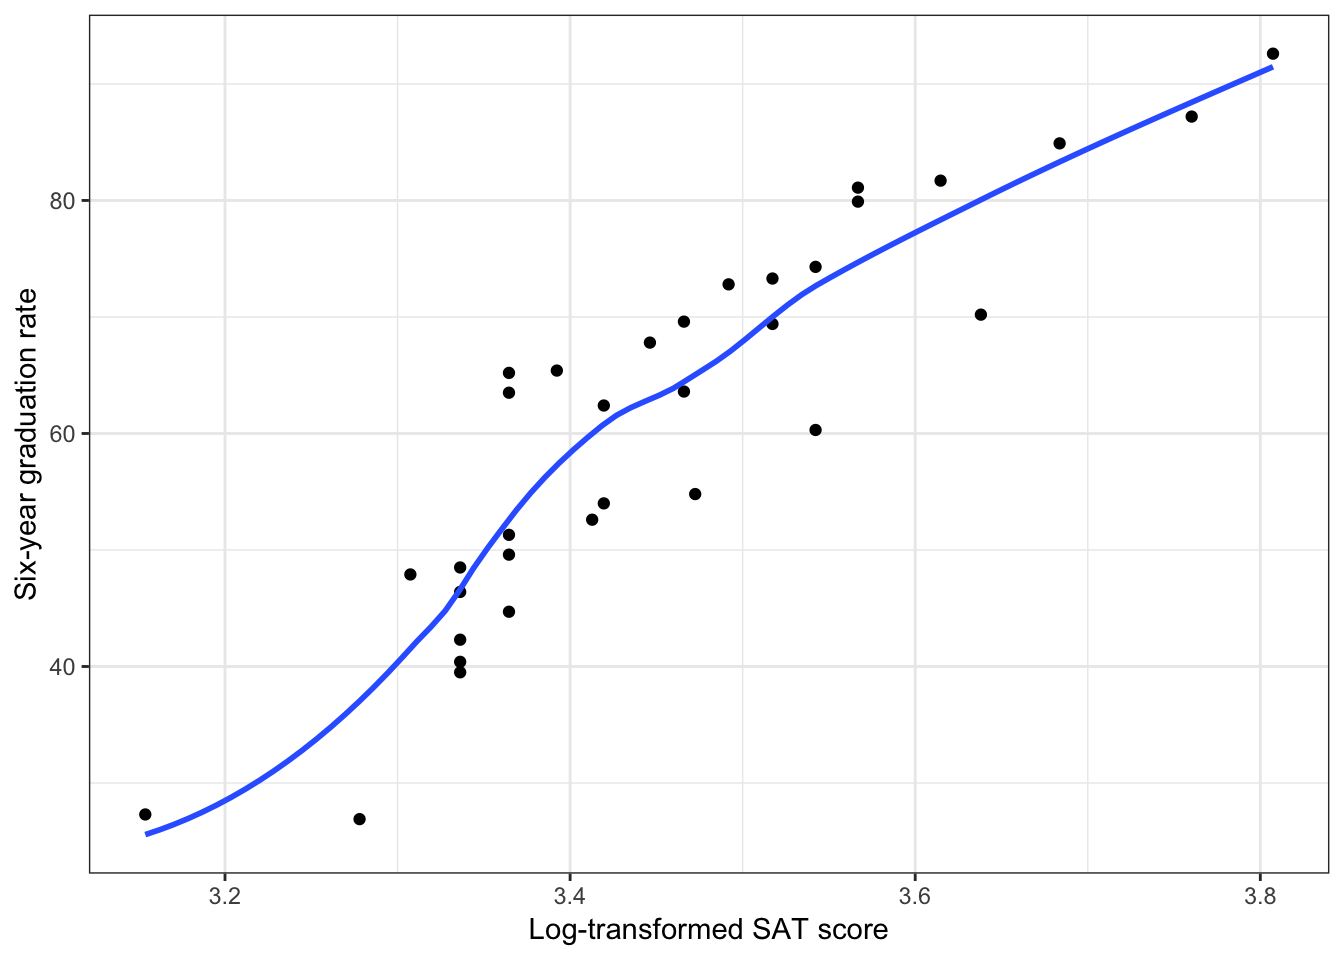
\includegraphics[width=0.5\linewidth]{bookdown-demo_files/figure-latex/unnamed-chunk-9-1} \caption{Scatterplot displaying the relationship between employee education levels and incomes. The OLS fitted regression line is also displayed.}\label{fig:unnamed-chunk-9}
\end{figure}

Consider all the employees that have an education level of 10 years. For
all three of them we would predict an income of approximately \$37,800.
This is denoted by the blue point on the line. The error term allows for
discrepancy between the predicted \(Y\) and the observed \(Y\), which
allows us to recover our observed value of the response variable from
the model.

Graphically, the residual is represented by the vertical distance
between the line and a given point on the scatterplot. Some of those
points are above the line (they have a positive residual) and some are
below the line (they have a negative residual). Also note that for some
observations the error term is smaller than for others.

\hypertarget{notation}{%
\subsection{Notation}\label{notation}}

The regression model and the fitted regression equation describe the
linear relationship in the \emph{population}. Greek letters indicate a
\emph{parameter} (a summary of the population). That is why we use the
Greek letters \(\beta\) and \(\epsilon\) when we notate the regression
model.

In most statistical analyses, you will use a \emph{sample} of data (not
the entire population). When we summarize a sample, it is referred to as
a \emph{statistic}, and we use either Roman letters or a Greek letter
with a hat. This indicates that the summary measure is an estimate of
the parameter. For example, the values produces for the intercept and
slope from a regression analysis are estimates. Since they are
estimates, we use the hat-notation on the greek letters.

\[
\hat{Y}_i = \hat{\beta}_0 + \hat{\beta}_1(X_i)
\]

The parameter estimates are also referred to as regression coefficients.
Synonymously, a hat means estimated/predicted value. Some people use
Roman letters when referring to sample estimates.

\[
\hat{Y}_i = B_0 + B_1(X_i)
\]

Similarly, in the population the error terms are expressed as the Greek
letter epsilon (\(\epsilon_i\)), while in the sample we use the Roman
letter e (\(e_i\)). The sample errors are also referred to as
\emph{residuals}.

\hypertarget{estimating-the-regression-coefficients-using-r}{%
\section{Estimating the Regression Coefficients Using
R}\label{estimating-the-regression-coefficients-using-r}}

To fit the regression model to data using R, we will use the
\texttt{lm()} function. The syntax for this function looks like this:

\begin{quote}
\texttt{lm(}\textbf{outcome} \textasciitilde{} \texttt{1\ +}
\textbf{predictor}, \texttt{data\ =} \textbf{dataframe}\texttt{)}
\end{quote}

where \textbf{outcome} is the name of the outcome/response variable,
\textbf{predictor} is the name of the predictor variable, and
\textbf{dataframe} is the name of the data frame. (The one on the right
side of the tilde tells R to include the intercept in its computation.)
When we fit a regression model in R, we will also assign the output to a
new object in R. Below, we fit the model using education level to
predict income.

\begin{Shaded}
\begin{Highlighting}[]
\NormalTok{lm}\FloatTok{.1}\NormalTok{ =}\StringTok{ }\KeywordTok{lm}\NormalTok{(income }\OperatorTok{~}\StringTok{ }\DecValTok{1} \OperatorTok{+}\StringTok{ }\NormalTok{education, }\DataTypeTok{data =}\NormalTok{ city)}
\end{Highlighting}
\end{Shaded}

Here the output is assigned to an object called \texttt{lm.1}. We can
print the regression parameter estimates by typing the \texttt{lm()}
object name and hitting enter.

\begin{Shaded}
\begin{Highlighting}[]
\NormalTok{lm}\FloatTok{.1}
\end{Highlighting}
\end{Shaded}

\begin{verbatim}
## 
## Call:
## lm(formula = income ~ 1 + education, data = city)
## 
## Coefficients:
## (Intercept)    education  
##      11.321        2.651
\end{verbatim}

Here the parameter estimates (or regression coefficients) are:

\begin{itemize}
\tightlist
\item
  \(\hat{\beta}_0 = 11.32\)
\item
  \(\hat{\beta}_1 = 2.65\)
\end{itemize}

The fitted regression equation is

\[
\hat{\mathrm{Income}}_i = 11.32 + 2.65(\mathrm{Education~Level}_i).
\]

\hypertarget{intercept-interpretation}{%
\subsection{Intercept Interpretation}\label{intercept-interpretation}}

The estimate for the intercept was 11.32. Graphically, this value
indicates the \(y\)-value where the line passes through the \(y\)-axis
(i.e., \(y\)-intercept). As such, it gives the predicted value of \(Y\)
when \(X = 0\). Algebraically we get the same thing if we substitute 0
in for \(X_i\) in the estimated regression equation.

\[
\begin{split}
\hat{Y}_i &= \hat{\beta}_0 + \hat{\beta}_1(0) \\
\hat{Y}_i &= \hat{\beta}_0 
\end{split}
\]

In our example,

\[
\begin{split}
\hat{Y}_i &= 11.32 + 2.65(0) \\
\hat{Y}_i &= 11.32 
\end{split}
\]

To interpret this value, we use that same idea. Namely

\begin{quote}
The predicted income for all employees that have an education level of 0
years is 11.32 thousand dollars.
\end{quote}

\hypertarget{slope-interpretation}{%
\subsection{Slope Interpretation}\label{slope-interpretation}}

Recall from algebra that the slope of a line describes the change in
\(Y\) versus the change in \(X\). In regression, the slope describes the
\emph{predicted} change in \(\hat{Y}\) for a one-unit difference in
\(X\).

\[
\hat{\beta}_1 = \frac{\Delta\hat{Y}}{\Delta X} = \frac{2.65}{1}
\]

In our example,

\begin{quote}
Each one-year difference in education level is associated with a 2.65
thousand dollar predicted difference in income.
\end{quote}

To better understand this, consider three city employees. The first
employee has an education level of 10 years. The second has an education
level of 11 years, and the third has an education level of 12 years. Now
let's compute each employee's predicted income.

\[
\begin{split}
\mathbf{Employee~1:~}\hat{\mathrm{Income}} &= 11.32 + 2.65(10) \\
&= 37.82
\end{split}
\]

\[
\begin{split}
\mathbf{Employee~2:~}\hat{\mathrm{Income}} &= 11.32 + 2.65(11) \\
&= 40.47
\end{split}
\]

\[
\begin{split}
\mathbf{Employee~3:~}\hat{\mathrm{Income}} &= 11.32 + 2.65(12) \\
&= 43.12
\end{split}
\]

Each of the employee's education levels differ by one year (10 to 11 to
12). The difference in predicted incomes for these employees differs by
2.65 thousand dollars.

\hypertarget{using-the-regression-equation}{%
\section{Using the Regression
Equation}\label{using-the-regression-equation}}

Consider the first case in the data frame.

\begin{Shaded}
\begin{Highlighting}[]
\NormalTok{city }\OperatorTok
\StringTok{  }\KeywordTok{filter}\NormalTok{(}\KeywordTok{row_number}\NormalTok{() }\OperatorTok{==}\StringTok{ }\DecValTok{1}\NormalTok{)}
\end{Highlighting}
\end{Shaded}

\begin{verbatim}
## # A tibble: 1 x 6
##   education income seniority gender  male party   
##       <int>  <dbl>     <int> <chr>  <int> <chr>   
## 1         8   37.4         7 male       1 Democrat
\end{verbatim}

This employee has an education level of eight years (\(X_{1}=8\)). His
income is 37.45 thousand dollars (\(Y_{1}=37.45\)). Using the fitted
equation, we can compute that employee's predicted income as,

\begin{Shaded}
\begin{Highlighting}[]
\FloatTok{11.32} \OperatorTok{+}\StringTok{ }\FloatTok{2.65} \OperatorTok{*}\StringTok{ }\DecValTok{8}
\end{Highlighting}
\end{Shaded}

\begin{verbatim}
## [1] 32.52
\end{verbatim}

\(\hat{Y}_{12} = 32.52\).

We can also compute that employee's residual.

\begin{Shaded}
\begin{Highlighting}[]
\FloatTok{37.45} \OperatorTok{-}\StringTok{ }\FloatTok{32.52}
\end{Highlighting}
\end{Shaded}

\begin{verbatim}
## [1] 4.93
\end{verbatim}

\(e_{1} = 4.93\).

The positive residual suggests that this employee earns 4.93 thousand
dollars more than would be expected for a city employee with eight years
of formal education. We can also represent these values graphically.

\begin{figure}
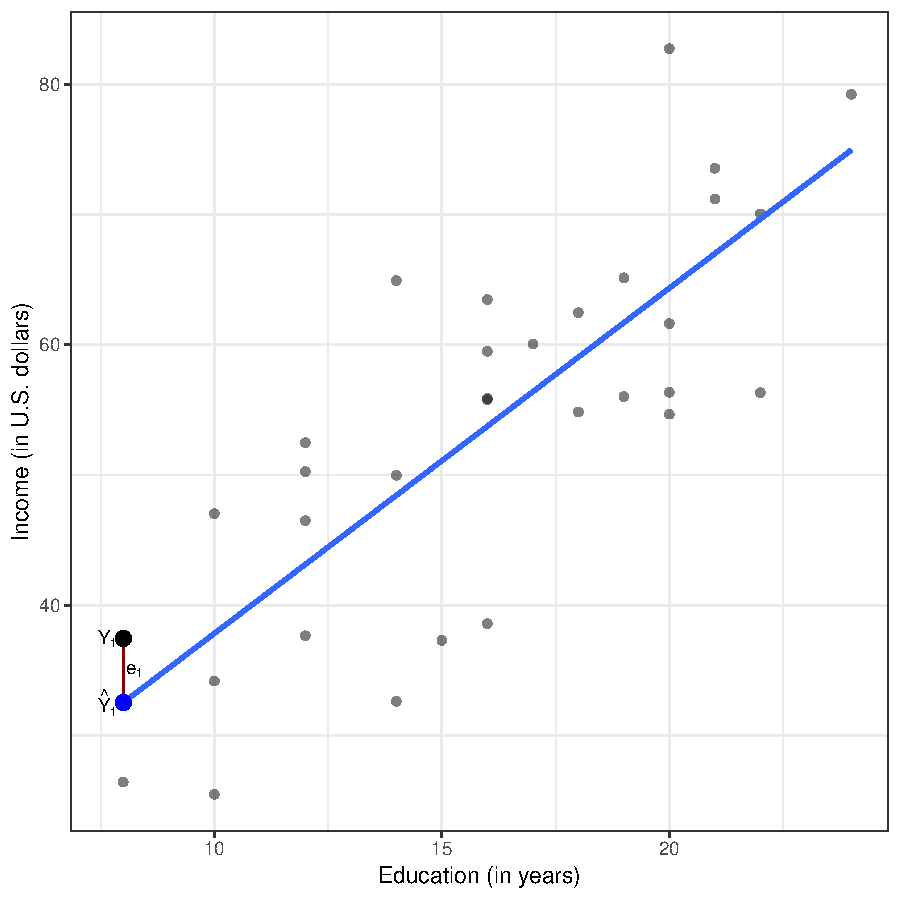
\includegraphics[width=0.5\linewidth]{bookdown-demo_files/figure-latex/unnamed-chunk-15-1} \caption{Plot displaying the OLS fitted regression line (blue) between employee education levels and incomes. The first employee's observed data (black dot) is plotted, and a visual representation of the employee's residual (red line) is also displayed.}\label{fig:unnamed-chunk-15}
\end{figure}

\hypertarget{conditional-averages}{%
\section{Conditional Averages}\label{conditional-averages}}

To this point, we have used the fitted regression equation to predict
for individual employees. Another way to think about the predicted value
is it describes the mean value of \(Y\) for \emph{all} cases with a
particular \(X\) value. For example, using the values from the previous
example we found that \(\hat{Y}_{1} = 37.45\) when \(X_{1}=8\). Using
means, we could interpret this as,

\begin{quote}
The estimated average income for city employees having 8 years of
education is 37.45 thousand dollars.
\end{quote}

A statistician may refer to the predicted value of \(Y\) as a
conditional mean (it is conditioned on a particular value of \(X\)). To
help better understand the idea of conditional means, consider the
following plot:

\begin{figure}
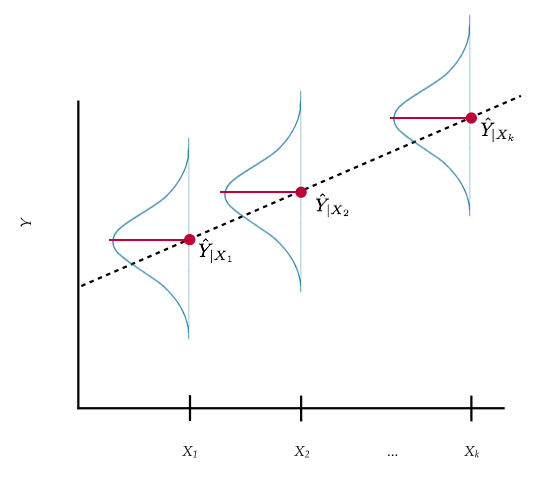
\includegraphics[width=0.5\linewidth]{images/conditional-means} \caption{Plot displaying conditional distribution of $Y$ at several $X$ values. The OLS fitted regression line (dotted) is also shown. The red points show the mean value of $Y$ for each conditional distribution.}\label{fig:unnamed-chunk-16}
\end{figure}

Examining this plot, we see at each value of \(X\) there is a
distribution of \(Y\). For example, there would be a distribution of
incomes for the employees with an education level of 8 years (in the
population). There would be another distribution of incomes for the
employees with an education level of 9 years (in the population). And so
on.

The regression equation describes the pattern of conditional means. As
such, we can write the fitted equation using means rather than
\(\hat{Y}\),

\[
\mu_{Y|X_i} = \beta_0 + \beta_1(X_i)
\]

The first part is read as, ``the mean of \(Y\) given \(X_i\)'', or ``the
mean of \(Y\) conditioned on \(X_i\)''. Sometimes the mean of a
population is denoted as \(E(Y)\), or the expected value of \(Y\). Then
you might see the regression equation written as,

\[
E(Y|X_i) = \beta_0 + \beta_1(X_i)
\]

When we assume a linear functional form for the model, we are saying
that the mean value of \(Y\) differs by a constant amount for each
one-unit difference in \(X\). In other words, the difference between the
mean income for those employees who have ten years of education and
those that have 11 years of education \emph{is the same as} the
difference between the mean income for those employees who have 17 years
of education and those that have 18 years of education.

Using this idea, the statistical model can be written as,

\[
\begin{split}
Y_i &= \beta_0 + \beta_1(X_i) + \epsilon_i \\
Y_i &= \mu_{Y|X_i} + \epsilon_i
\end{split}
\]

That is, each observations observed value (\(Y_i\)) is a function of the
mean \(Y\)-value (given \(X_i\)) and error. The error represents how far
the observed value is from that mean:

\[
\epsilon_i  = Y_i - \mu_{Y|X_i}
\]

In statistical parlance, this is referred to as a \emph{mean deviation}.

\hypertarget{intercept-re-visited}{%
\subsection{Intercept (Re-visited)}\label{intercept-re-visited}}

Using the idea of conditional means, we can re-visit the interpretation
of the intercept, which we had said was the predicted \(Y\) for a person
with an \(X\)-value of zero. Now we can say that the intercept is the
predicted mean income for all employees with zero years of formal
education.

\begin{figure}
\includegraphics[width=0.5\linewidth]{images/conditional-means-interept} \caption{Plot displaying conditional distribution of $Y$ at $X=0$. The OLS fitted regression line (dotted) is also shown. The red points show the mean value of $Y$ for this conditional distribution---which corresponfds to the intercept value of the regression line.}\label{fig:unnamed-chunk-17}
\end{figure}

\hypertarget{slope-re-visited}{%
\section{Slope (Re-visited)}\label{slope-re-visited}}

Using the idea of conditional means, we can also re-visit the
interpretation of the slope, which we had said was the predicted
difference in \(Y\) for employees with a one-year difference in
education. Now we can say that the slope is the predicted difference in
mean incomes between employees with education levels that differ by one
year.

\begin{figure}
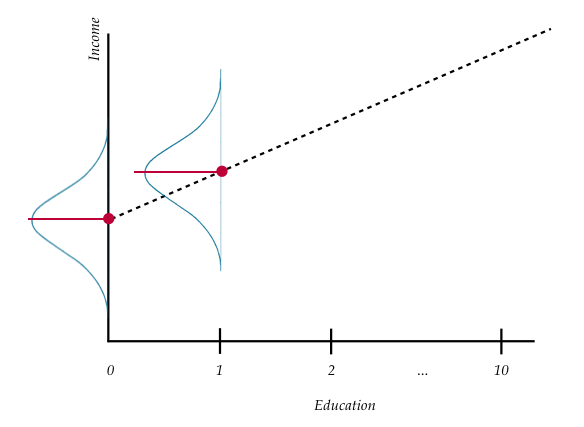
\includegraphics[width=0.5\linewidth]{images/conditional-means-slope} \caption{Plot displaying conditional distribution of $Y$ at $X=0$ and $X=1$. The OLS fitted regression line (dotted) is also shown. The red points show the mean value of $Y$ for these conditional distributions---the relative change which corresponfds to the slope value of the regression line.}\label{fig:unnamed-chunk-18}
\end{figure}

\begin{quote}
In general, when interpreting the slope and intercept, you should use
the conditional mean interpretations.
\end{quote}

\hypertarget{literature}{%
\chapter{Literature}\label{literature}}

Here is a review of existing methods.

\hypertarget{methods}{%
\chapter{Methods}\label{methods}}

We describe our methods in this chapter.

\hypertarget{applications}{%
\chapter{Applications}\label{applications}}

Some \emph{significant} applications are demonstrated in this chapter.

\hypertarget{example-one}{%
\section{Example one}\label{example-one}}

\hypertarget{example-two}{%
\section{Example two}\label{example-two}}

\hypertarget{final-words}{%
\chapter{Final Words}\label{final-words}}

We have finished a nice book.

\bibliography{epsy8251.bib}


\end{document}
